%%%%%%%%%%%%%%%%%%%%%%%%%%%%%%%%%%%%%%%%%%%%%%
%                insertmeeting
% 1) Title (something creative & funny?)
% 2) Date (MM/DD/YYYY)
% 3) Location (ex. Hagerty High School)
% 4) People/Committees Present 
% 5) Picture 
% 6) Start Time & Stop Time (ex. 12:30AM to 4:30PM)
%%%%%%%%%%%%%%%%%%%%%%%%%%%%%%%%%%%%%%%%%%%%%%
\insertmeeting 
	{Kinematics Katastrophe and Rapid Replacements} 
	{01/12/22} 
	{Hagerty High School}
	{Annika, Anouska, James, Nathan, Ritam, Samantha}
	{Images/RobotPics/robot.jpg}
	{2:30 - 4:30}
	
\hhscommittee{Software}
\noindent\hfil\rule{\textwidth}{.4pt}\hfil
\subsubsection*{Goals}
\begin{itemize}
    \item Finish creating TricycleKinematics.kt and TricycleDrive.kt  

\end{itemize} 

\noindent\hfil\rule{\textwidth}{.4pt}\hfil

\subsubsection*{Accomplishments}
When we started testing our new methods today, we ran into a few issues. The first problem was that when we told the robot to go to a certain position, it often ended up going the correct direction, but it always moved to little or too much. This meant that our kinematic equations for calculating the desired robot heading were correct. The first section we began to troubleshoot was the x and y localization equations. Instead of telling the robot to move autonomously, we tried to turn on the robot but leave the unpowered wheels. This would allow us to check our calculations based purely on wheel rotations and encoder positions. We then logged the estimated position as we moved the robot around the field by hand. Surprisingly, the x and y coordinates were extremely accurate - only off by about a centimeter at most. This slight variation was expected, since our wheels were bound to slip during movement. The lack of dead wheel encoders due to our use of a single control hub meant that this problem could not be solved with conventional methods. We may have to continue testing the robot movement to see if this is a large enough problem to warrant a redesign. The next piece that we decided to check was how we sent information to the motors in our "SetDriveSignal" function. Upon further inspection, we realized that we made a mistake in one of the lines. One of the calculations for the needed motor power was using a method from "TankKinematics", not the new "TricycleKinematics". After fixing this quick fix, the robot moved correctly from one point to another. 

\begin{figure}[htp]
\centering
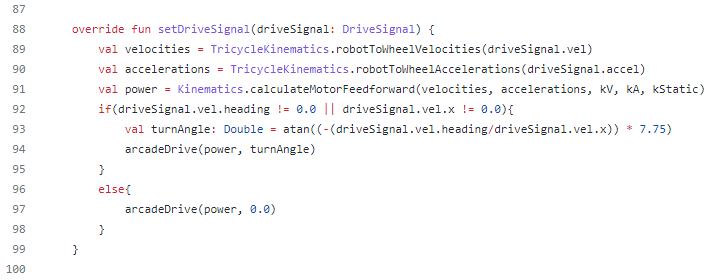
\includegraphics[width=0.95\textwidth, angle=0]{Meetings/January/01-12-22/1.12.22 drivesignal - James Hu.PNG}
\caption{Our modified driveSignal class that fixed the robot's incorrect movement}
\label{fig:011222_1}
\end{figure}


	
\hhscommittee{Hardware}
\noindent\hfil\rule{\textwidth}{.4pt}\hfil
\subsubsection*{Goals}
\begin{itemize}
    \item Make small change to intake sides


\end{itemize} 

\noindent\hfil\rule{\textwidth}{.4pt}\hfil

\subsubsection*{Accomplishments}
Today we are putting the modularity of our intake design to the test! After doing some driver practice, we started noticing that the intake had trouble grabbing elements if they weren't already centered with the intake. To improve our efficiency, we don't want to have to worry about lining up with a block. Instead , we would like to be able to simply drive into a pile of elements and have our intake automatically grab one for us. The reason for the elements not going in when they are slightly misaligned is because of the shape of our intake’s sides. Because they have a shallow angle supporting the spinner that sticks out towards the front, elements are blocked from being pulled in if they are a bit off to the side. We want to change this angle to be a rounded arch to reduce the bulk of the sides, while still supporting the sweeper well. To ensure that the sweeper is well supported, we also planned to add some more support on the top (Figure \ref{fig:011222_2}). Going into CAD we made these changes to the sides and changed the pocketing to ensure the models were strong and light (Figure \ref{fig:011222_3}). After cutting the sides out on the glowforge, we were able to easily screw the new parts on, as quickly and efficiently as we had hoped. While testing, we found that the new sides made some improvement on intaking blocks that aren’t lined up perfectly.


\begin{figure}[ht]
\centering
\begin{minipage}[b]{.48\textwidth}
  \centering
  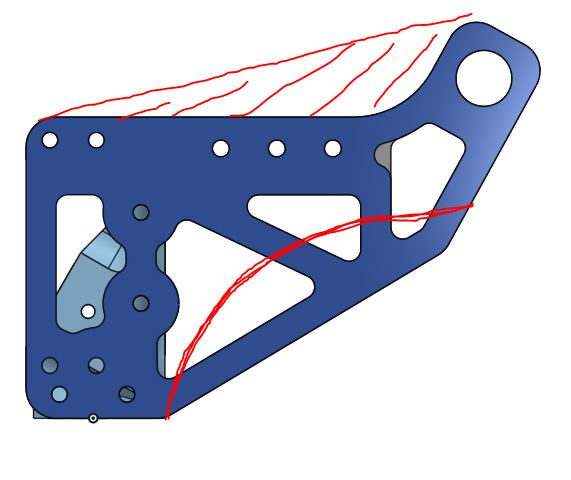
\includegraphics[width=0.95\textwidth]{Meetings/January/01-12-22/1-12-22_Hardware_Figure1 - Nathan Forrer.PNG}
  \caption{We plan to add more support}
  \label{fig:011222_2}
\end{minipage}%
\hfill%
\begin{minipage}[b]{.48\textwidth}
  \centering
  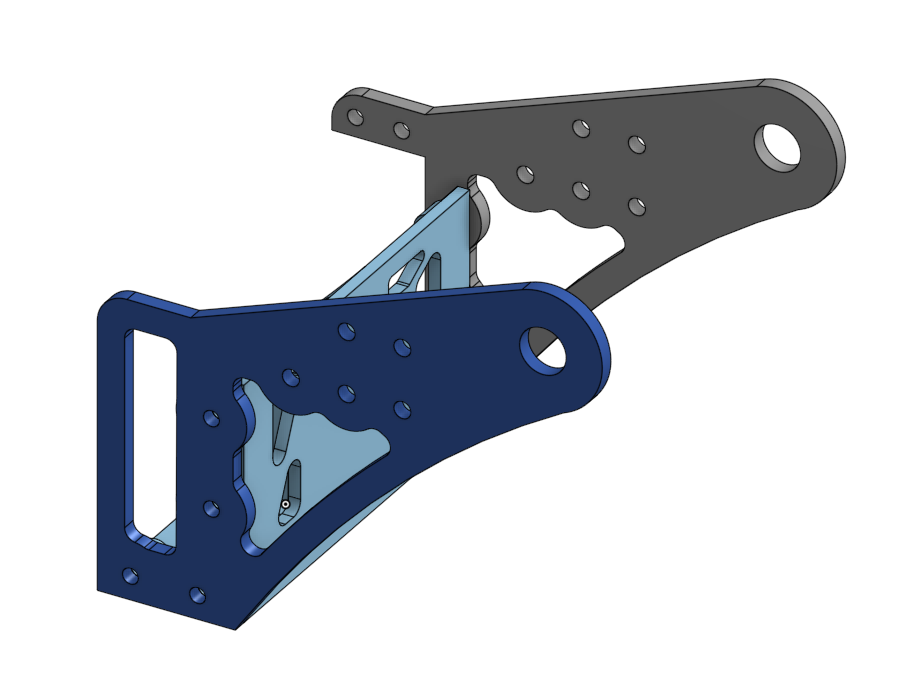
\includegraphics[width=0.95\textwidth]{Meetings/January/01-12-22/1-12-22_Hardware_Figure2 - Nathan Forrer.PNG}
  \caption{New pocketing}
  \label{fig:011222_3}
\end{minipage}
\end{figure}


\whatsnext{
\begin{itemize}
    \item Begin to integrate our new Road Runner Tricycle foundation into a TRC-event capable drivebase.
    \item make any other necessary hardware changes
	\item prepare for meet 3
\end{itemize} 
}

